\documentclass[11pt, a4paper]{article}

\usepackage{amsmath}
\usepackage{amssymb}
\usepackage{graphicx}
\usepackage{listings}
\usepackage{color}
\usepackage[section]{placeins}
\usepackage{paralist}
\usepackage{fullpage}
\usepackage{glossaries}
\usepackage{url}

\usepackage{caption}
\usepackage{subcaption}

\newcommand*{\titleGM}{\begingroup
\hbox{ 
\hspace*{0.2\textwidth} 
\rule{1pt}{\textheight} 
\hspace*{0.05\textwidth} 
\parbox[b]{0.75\textwidth}{ 

{\noindent\Huge\bfseries An Android Homepage Widget}\\[2\baselineskip] % Title
{\large \textit{SEM2220 Assignment 3}}\\[4\baselineskip] % Tagline or further description
{\Large \textsc{Alexander D Brown (adb9)}} % Author name

\vspace{0.5\textheight} 
}}
\endgroup}


\begin{document}
\titleGM 
\tableofcontents
\newpage

\section{Introduction}
This report details the process undertaken to produce an Android widget based 
on the existing code to load sessions from a SQLite database. This widget had 
several requirements, including the ability to select different days from the 
database as well as provide notifications read from a remote URL.

\section{Design}
The widget was designed in accordance with the Android App Widget Design 
Guidelines\cite{google2013widget}, which define guides for design constraints 
like the minimum and maximum size of the widget, layouts and backgrounds, etc.

To help conform to these guidelines, the template design 
pack\cite{google2013widgettemplates} provided by the Android Open Source 
Project under the Apache 2 License was used to design the widget. 

A mock version of the widget was created to view how it would appear on a 
device. From this is became obvious that the widget would need to be four 
cells wide (the maximum) by at least two cells tall.

This size would allow a view with the following information on it:

\begin{itemize}
  \item A title for the Widget
  \item Two buttons, one to move backwards through days and one to move forward
        through days
  \item A list of the sessions available for the specified day.
  \item The notification loaded from a remote site.
\end{itemize}

To keep the buttons accessible, they were made such that their minimum size was
a single cell each and surrounded the list of sessions to make the flow of data
natural. To conform to the iconography standards\cite{google2013iconography},
another resource was used from the Android Open Source Project; the Action Bar 
Icon Pack\cite{google2013iconpack}.

The notification display was kept small so that it would not obstruct the view
of the data, but so that it would be easy to see at a glance. Finally, the 
title was given colour, based on the recommended 
colours\cite{google2013colour}, a purely aesthetic element.

\begin{figure}[h]
\centering
\begin{subfigure}[h]{0.3\textwidth}
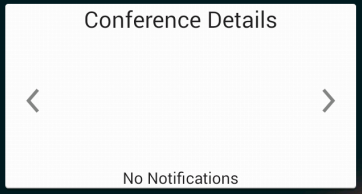
\includegraphics[width=\textwidth]{img/design_initial}
\caption{Initial Widget Design}
\end{subfigure}
\begin{subfigure}[h]{0.3\textwidth}
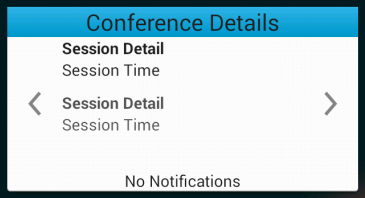
\includegraphics[width=\textwidth]{img/design_second}
\caption{Improved Widget Design}
\end{subfigure}
\begin{subfigure}[h]{0.3\textwidth}
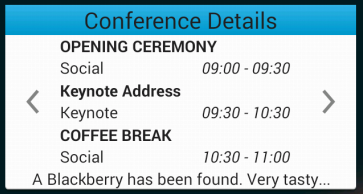
\includegraphics[width=\textwidth]{img/design_final}
\caption{Final Widget Design}
\end{subfigure}

\caption{Evolution of the Widget Design}
\label{fig:widget_design}
\end{figure}

Figure~\ref{fig:widget_design} shows the evolution of the design for the 
widget.


\section{Development}

Most of the development was based on the documentation of Android App 
Widget\cite{google2013appwidgets}. Following this resource, the API and some 
examples from both the Android Open Source Project and textbook codes 
samples\cite{murphy2009android}. With these resources it was a fairly simple 
matter to implement the basic widget.

All the development for the widget was kept in a separate Android project. The
first action was to import the \texttt{DataAccess} class provided into this 
project. The next step was to create a class which implemented 
\texttt{AppWidgetProvider}. This used the layout shown in the previous section
and a \texttt{RemoteViews} object to manipulate the elements in that layout.

To enable the loading of list content, subclasses \texttt{RemoteViewsService} 
and \texttt{RemoteViewsFactory} were created. The service simply provides this 
factory, whilst the service loads content into the list from the SQLite3 
database using the \texttt{DataAccess} class.

This brought forward a problem; the SQLite3 table row IDs defined in
\texttt{ConferenceCP} did not match the actual SQLite3 row IDs provided. This
lead to incorrect data being provided by the \texttt{DataAccess} class. Fixing
this was a simple matter of changing these IDs to match the right IDs, but this
may not apply to other implementations of SQLite3 (the version exported works
in SQLite version 3.7.11, on the Android Emulator running on Linux Mint 14 
Cinnamon 64-bit).

To improve the loading of Sessions, a POJO\cite{fowler2000pojo} was created to
represent a session and an additional method for loading this POJO was added 
into the \texttt{DataAccess} class. The same thing was created to load a Date
object from the database as the Session requires this. With these POJOs it was
easy to display this in the list rows.

The next task was to implement the next day and previous day functionality. 
Initially the code for this was doing the widget provider. The buttons would 
send a broadcast (either next or previous) to the provider and then to forcibly
call the \texttt{onUpdate} method to reset the broadcasts and list service.

However, talking to a fellow classmate (Gareth Williams) the easier way to do
this was to send a broadcast to the service directly and just notify the App
Widget Manager that the data for the list had changed.

Finally, to download the notification an \texttt{AsyncTask} was implemented to
handle the URL connection as it cannot be done in the Android main thread. The
code for this is fairly standard and the correct permissions had to be set in
the manifest file.


\section{Testing}
All testing was performed using the Android emulator. Most of this testing
involved using the widget to ensure it worked correctly. Actually unit testing
the code would have been fairly trivial as it only really integrated existing
code and displayed it in layouts.

All figures below show the widget running on an emulated Nexus 4 at API level 
19 (Android 4.4). The widget should also function on any API level 14 and above
(Android 4.X). This is a requirement for the loading of the list.

Figure~\ref{fig:days} shows the widget running on the emulator displaying 
information for all sessions on the three days. 

\begin{figure}[h]
\centering
\begin{subfigure}[b]{0.3\textwidth}
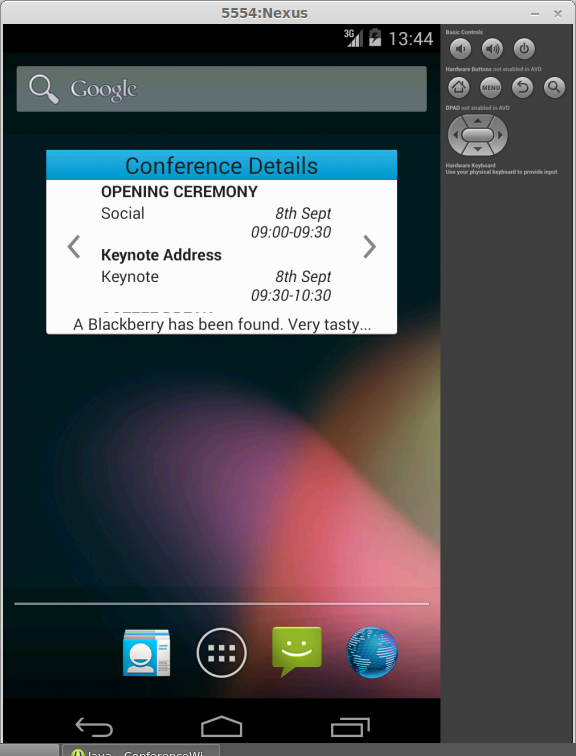
\includegraphics[width=\textwidth]{img/running-day-1.png}
\caption{The first day}
\end{subfigure}
\begin{subfigure}[b]{0.3\textwidth}
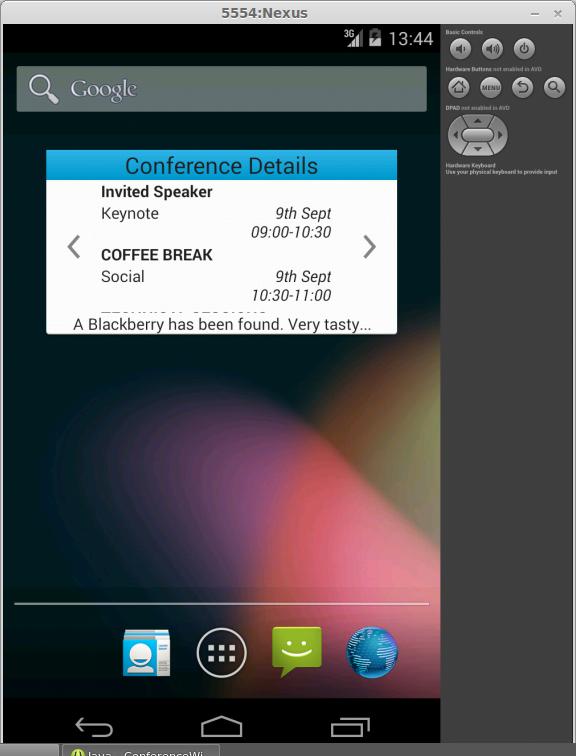
\includegraphics[width=\textwidth]{img/running-day-2.png}
\caption{The second day}
\end{subfigure}
\begin{subfigure}[b]{0.3\textwidth}
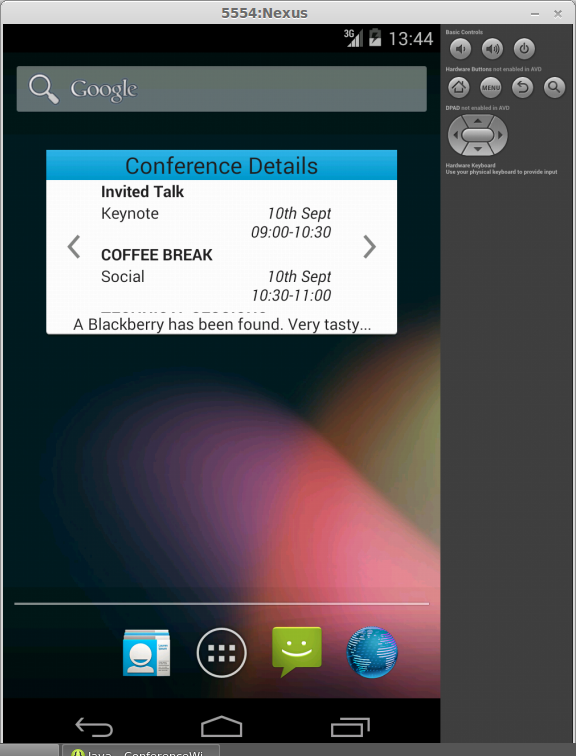
\includegraphics[width=\textwidth]{img/running-day-3.png}
\caption{The third day}
\end{subfigure}
\caption{The Widget displaying session information for the three different 
         days}
\label{fig:days}
\end{figure}

Figure~\ref{fig:resize} shows the widget's ability to resize vertically to show
more information, depending on the user's available space.

\begin{figure}[h]
\centering
\begin{subfigure}[b]{0.3\textwidth}
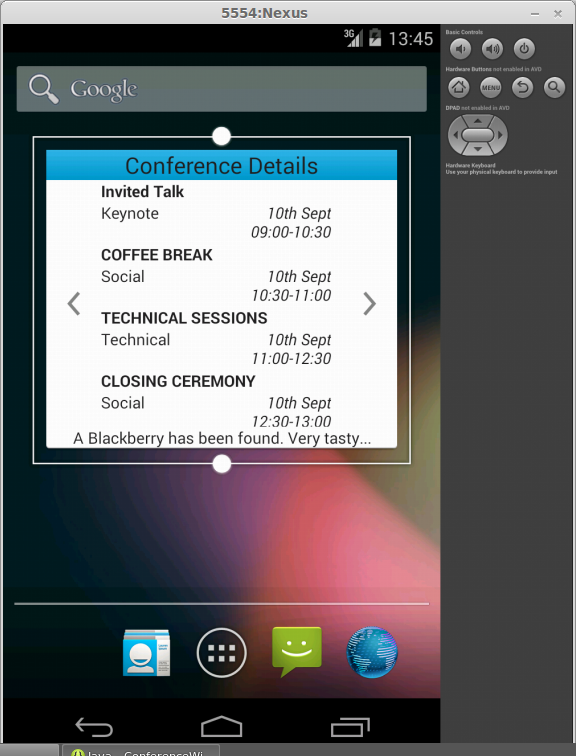
\includegraphics[width=\textwidth]{img/resizing-3x4}
\caption{Resizing to 3 by 4 cells}
\end{subfigure}
\begin{subfigure}[b]{0.3\textwidth}
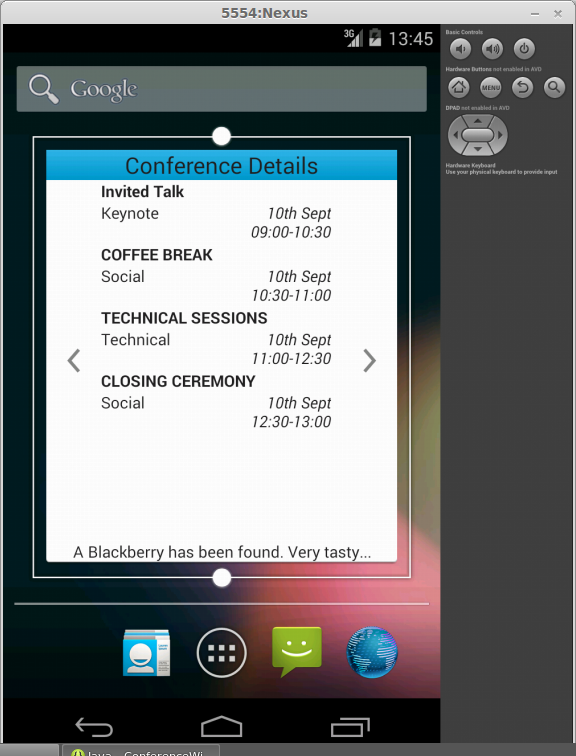
\includegraphics[width=\textwidth]{img/resizing-4x4}
\caption{Resizing to 4 by 4 cells}
\end{subfigure}
\caption{Resizing the widget to show more information}
\label{fig:resize}
\end{figure}

Figure~\ref{fig:notification} shows that the widget will dynamically load a 
different notification from the remote URL.

\begin{figure}[h]
\centering
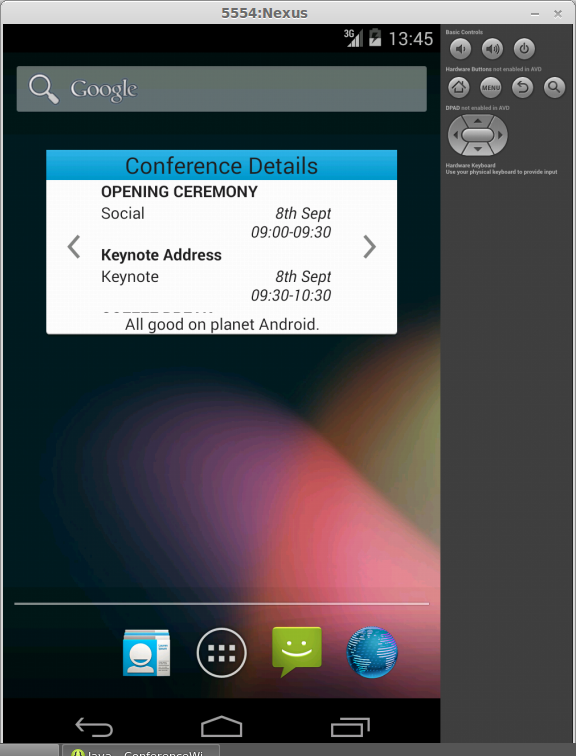
\includegraphics[width=0.3\textwidth]{img/new-notification}
\caption{Proving that the widget will load a new notification.}
\label{fig:notification}
\end{figure}

\section{Evaluation}

All of the feature requests have been implemented and evidenced as per the 
figures shown in the previous section. The code is of decent quality and 
conforms to the Android developer guidelines.

The author has learned about the creation of Android homescreen widgets, having
successfully implemented one, and has found the process to be challenging but 
not unduly difficult. One does wonder why the Android API has such good support
for Activities and Services, but how the implementation of widgets feels 
somewhat mixed, surely a base class like Activity could have been provided to 
handle widgets rather than directly manipulating remote views.

A lot of the time spent on this project was spent understanding this 
architecture and figuring out how to handle certain events correctly. It does 
have the feeling that the actions to go left and right were not the kind of
operation that widgets are meant to perform. But trying to implement this in a
different way, by using a stacked view, lead to the problem that the lists
could not be generated correctly inside another view.

The amount of documentation for widgets is limited, so the example found in the
book\cite{murphy2009android} were a lot of help.

Aside from this, the normal numbers of error produced by either null pointers
or going beyond lists were encountered and fixed, though it would have been 
nice to debug the code using a debugger, but despite numerous attempts it would
not halt at breakpoints, despite the debugger being correctly attached. The
author would guess that widgets are so tied to the homescreen that it is 
difficult for the Android Operating System to unlink them.

Loading from a remote URL was a task the author has already investigated so did
not provide many problems, although the initial use of a 
\texttt{HttpURLConnection} and a \texttt{BufferedReader} did not combine well
and always resulted in empty content, despite the result being 
\texttt{HTTP 1.1/200 OK}. The solution was to simplify this and use the simpler
\texttt{URLConnection} and \texttt{InputStreamReader}, manually setting the 
buffer size to 255; a value which should not take up too much RAM
of the device, but which should be enough to load the data quickly.


Breaking down the mark scheme the author has predicted the grade which should 
be given for each part, this is shown in table~\ref{tab:marks}.

Therefore, the author feels a mark of 86\% should be awarded. The values chosen 
were based on the following reasons:

\begin{description}
\item[Documentation] This report conveys a detailed story of the implementation
                     of code, problems encountered, lessons learned and this 
                     indication of the mark which should be awarded.
\item[Implementation] The design and code meets the specified functionality and
                      conforms to the Android development guidelines.
\item[Flair] The code has been implemented in a maintainable and proper manner,
             especially in using POJOs to handle database interaction. The use
             of a list to display sessions is also a complex feature which the
             specification did not ask for.
\item[Testing] Evidence of testing on the Android emulator has been provided.
\end{description}

\begin{table}[h]
\centering
\begin{tabular}{|c|c|c|}\hline
\textbf{Part} & \textbf{Worth} & \textbf{Predicted Grade} \\ \hline
Documentation & 30\% & 27\% \\ 
Implementation & 50\% & 45\% \\ 
Flair & 10\% & 7\% \\ 
Testing & 10\% & 7\% \\ \hline
Total & 100\% & 86\% \\ \hline
\end{tabular}
\caption{Break Down of Marks}\label{tab:marks}
\end{table}

\newpage

\bibliographystyle{IEEEtran}
\bibliography{bibliography}

\end{document}
